\documentclass[11pt,a4paper]{article}

\usepackage[margin=1in]{geometry}
\usepackage[T1]{fontenc}
\usepackage[utf8]{inputenc}
\usepackage{lmodern}
\usepackage{microtype}
\usepackage{amsmath,amssymb}
\usepackage{graphicx}
\usepackage{booktabs}
\usepackage{caption}
\usepackage{enumitem}
\usepackage{tikz}
\usetikzlibrary{positioning,arrows.meta,fit,backgrounds}
\usepackage[colorlinks=true,linkcolor=black,citecolor=blue!50!black,urlcolor=blue!50!black]{hyperref}

\setlist{itemsep=2pt,topsep=4pt}
\graphicspath{{figures/}}

\title{\textbf{Visus: Text-Guided Face Occlusion Segmentation\\using CLIP-based Cross-Modal Attention Fusion}}
\author{
  Arpita Deshmukh \qquad Sreenitya Thatikunta\\[4pt]
  \normalsize Indian Institute of Technology Jodhpur
}
\date{Computer Vision course project \quad\textbullet\quad April 2026}

\begin{document}
\maketitle

\begin{abstract}
Segmentation of facial occlusions (e.g., glasses and face masks) is a key challenge in building
robust face analysis and face detection systems. Existing approaches are mostly vision-only, which
limits their ability to capture high-level semantic concepts that are naturally expressed in language.
In this work, we introduce a cross-modal attention framework that integrates visual and textual
representations to improve fine-grained occlusion segmentation.

Our approach leverages a pre-trained CLIP (Contrastive Language--Image Pre-training) model to bridge
the gap between pixel-level visual features and semantic descriptions that come from text.
Specifically, we reinterpret transformer attention maps as spatial priors and align them with
text-derived representations, which helps the model localise semantically meaningful regions
corresponding to occlusions. We propose a Cross-Modal Attention Fusion mechanism that facilitates
structured interaction between visual attention and language embeddings, allowing the model to refine
predictions using complementary cross-modal cues. This design improves the model's ability to segment
the image in challenging cases where visual signals alone are insufficient.
\end{abstract}

% ---------------------------------------------------------------------------
\section{Introduction}

Face analysis is a fundamental component of applications such as biometric authentication and
surveillance. A persistent challenge in these systems is handling facial occlusions, where regions of
the face are partially covered by objects such as eyeglasses or masks. Such occlusions corrupt the
feature representations extracted by face encoders and can significantly degrade recognition
performance. Accurately localising occluded regions as binary masks can therefore serve as an
important pre-processing step for improving robustness.

Most existing approaches treat occlusion segmentation as a purely visual task. However, this overlooks
the fact that occlusions are inherently semantic: categories such as ``glasses'' or ``face mask'' carry
strong priors about shape, appearance, and spatial location. These priors are naturally encoded in
language and can complement visual features, especially in settings with limited supervision. Recent
vision--language models such as CLIP~\cite{radford2021clip} learn aligned representations across
modalities, providing a natural foundation for incorporating such semantic understanding into dense
prediction tasks.

In this work, we propose a framework that uses vision--language alignment to improve facial occlusion
segmentation. Our key idea is to reinterpret internal attention representations from a pre-trained
multimodal model as spatial priors, and to refine them through structured interaction with
text-derived features. This enables the model to incorporate high-level semantic guidance while
preserving fine-grained spatial detail.

% ---------------------------------------------------------------------------
\section{Related Work}

\paragraph{Transformer-based segmentation.}
Early work on image segmentation relied on fully convolutional networks (FCNs)~\cite{long2015fcn},
which enabled pixel-wise prediction directly from convolutional features. This idea was improved by
encoder--decoder architectures such as U-Net~\cite{ronneberger2015unet}, which combine low-level and
high-level features for better localisation. More recently, Vision Transformers
(ViT)~\cite{dosovitskiy2021vit} have shown that attention-based models can match or exceed
convolutional networks on visual tasks. Methods such as SETR~\cite{zheng2021setr} and
Segmenter~\cite{strudel2021segmenter} extend Vision Transformers to segmentation by operating on
sequences of patch tokens with dedicated decoders. We also use ViT-based features, but instead of
building a full decoder we use CLS-token attention maps as a simple spatial cue.

\paragraph{Attention maps as segmentation cues.}
Attention maps from transformers often highlight semantically meaningful regions.
DINO~\cite{caron2021dino} showed that self-supervised Vision Transformers exhibit emergent object
localisation, with attention maps roughly corresponding to foreground objects despite the absence of
labels. Chefer et al.~\cite{chefer2021interpretability} proposed relevance-based attribution for
transformers, which can be adapted to obtain spatial importance maps, and
Grad-CAM~\cite{selvaraju2017gradcam} uses gradients to localise important regions in CNNs. Inspired
by these works, we use the CLS-to-patch attention of the final transformer layer as a coarse estimate
of object regions, which is then refined by a lightweight segmentation module.

\paragraph{Vision--language models for localisation.}
CLIP~\cite{radford2021clip} learns a shared embedding space for images and text, enabling zero-shot
classification and retrieval. CLIPSeg~\cite{luddecke2022clipseg} adds a text-conditioned decoder for
language-guided segmentation; GroupViT~\cite{xu2022groupvit} and OVSeg~\cite{liang2023ovseg} extend
this to open-vocabulary segmentation, and Grounded-SAM~\cite{ren2024groundedsam} combines grounding
models with segmentation systems for text-driven queries. In contrast, our method is simpler and more
focused: rather than relying on heavy decoders, we fuse text features with visual attention maps using
lightweight modules.

\paragraph{Face occlusion handling.}
Occlusion in face analysis has been addressed with part-based and mask-learning
models~\cite{song2019occlusion} and mask-aware recognition~\cite{wang2020masked}, as well as
inpainting and attention-based methods that down-weight occluded features. Our approach instead
identifies occluded regions explicitly via segmentation, which can serve as a pre-processing step for
downstream recognition or reconstruction.

% ---------------------------------------------------------------------------
\section{Occluded Dataset Construction}

No large-scale public dataset provides pixel-level annotations for common occlusions such as glasses
and face masks, so we construct a synthetic dataset based on CelebA~\cite{liu2015celeba}.
Figure~\ref{fig:pipeline} illustrates the pipeline.

\begin{figure}[t]
  \centering
  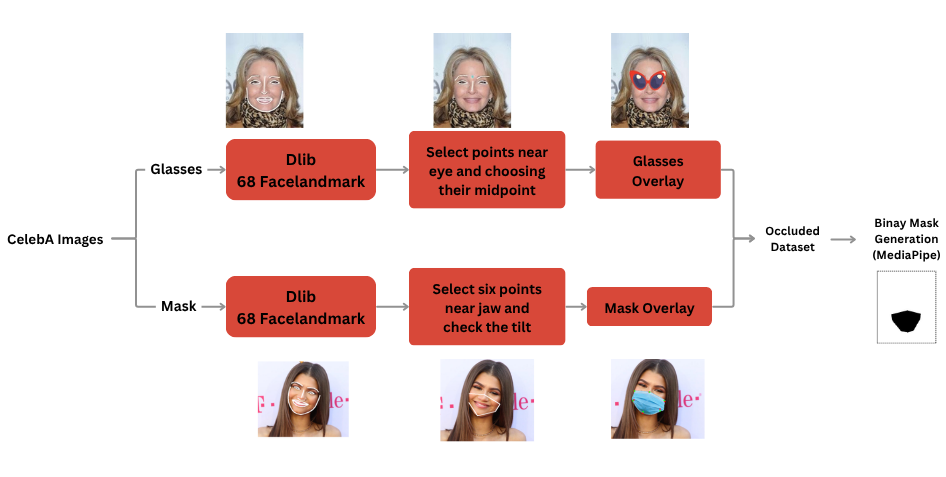
\includegraphics[width=\linewidth]{dataset_pipeline.png}
  \caption{Synthetic occlusion dataset construction. Facial landmarks are detected on CelebA images,
  glasses or masks are overlaid, and the corresponding binary segmentation masks are generated.}
  \label{fig:pipeline}
\end{figure}

\subsection{Base images}
CelebA contains over 200{,}000 images of 10{,}177 identities (about 20 images each) covering a wide
range of poses and lighting conditions, making it a suitable base for realistic occlusions.

\subsection{Synthetic occlusion augmentation}
\begin{itemize}
  \item \textbf{Glasses.} Eyeglasses and sunglasses are added with OpenCV. Facial landmarks (dlib, 68
  points) locate the eye region, and the glasses are resized and positioned to align with the face.
  \item \textbf{Face masks.} Masks are applied with the MaskTheFace framework~\cite{anwar2020maskedface},
  which places realistic mask overlays based on facial landmarks so that masks conform to facial
  structure across poses.
\end{itemize}

\subsection{Ground-truth mask generation}
Ground-truth masks are produced with MediaPipe Face Mesh~\cite{lugaresi2019mediapipe}. The detected
landmarks define the occluded region (the eye region for glasses, the lower face for masks), which is
rasterised into a binary mask.

\subsection{Text label assignment}
Each image is paired with a text label describing the occlusion. Instead of a single fixed label, each
category has a small set of semantically similar prompts, and one is sampled at random for every
training example to improve robustness to phrasing:
\begin{itemize}
  \item \textbf{Glasses:} ``Glasses'', ``Sunglass'', ``Eyewear'', ``Covered eyes'', ``Occluded eyes''
  \item \textbf{Face mask:} ``Mask'', ``Face mask'', ``Covered face'', ``Occluded region'', ``Non face region''
  \item \textbf{Clear face:} ``Face'', ``Human face'', ``Visible face'', ``Uncovered face'', ``Clear face region''
\end{itemize}

% ---------------------------------------------------------------------------
\section{Method}

Given an input image and a text prompt (e.g.\ ``glasses'' or ``face mask''), the image is processed by
the CLIP visual encoder and the prompt by the CLIP text encoder. From these two branches we extract
attention-based features: the visual attention map gives a coarse localisation of relevant regions,
and the text features give semantic context. The two are fused by cross-modal attention modules inside
a segmentation head that produces the final mask. Figure~\ref{fig:architecture} gives an overview.

\begin{figure}[t]
\centering
\resizebox{\linewidth}{!}{%
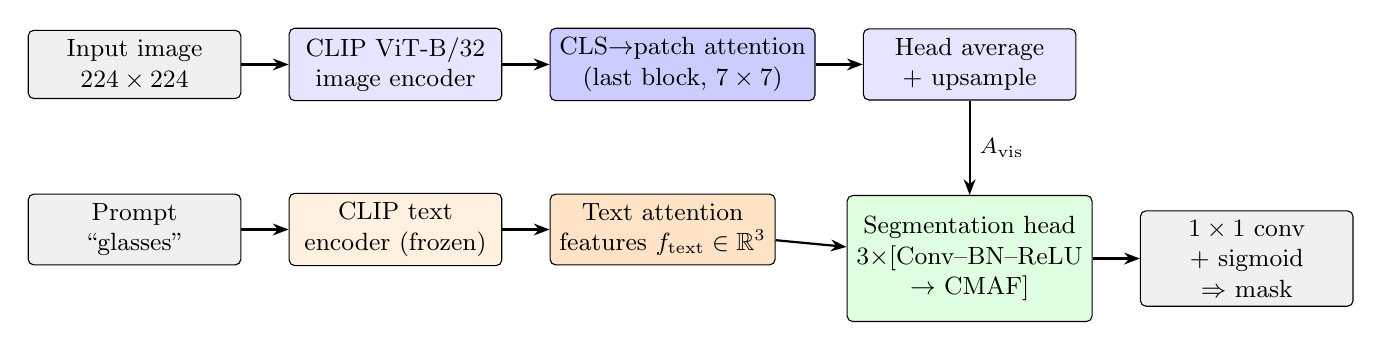
\begin{tikzpicture}[
  font=\small,
  box/.style={draw, rounded corners=2pt, align=center, minimum height=7mm, minimum width=27mm, fill=#1},
  box/.default=white,
  arr/.style={-{Stealth[length=2mm]}, thick},
  node distance=4mm and 6mm]

  % vision branch
  \node[box=gray!12] (img) {Input image\\$224\times224$};
  \node[box=blue!10, right=of img] (vit) {CLIP ViT-B/32\\image encoder};
  \node[box=blue!20, right=of vit] (attn) {CLS$\to$patch attention\\(last block, $7\times7$)};
  \node[box=blue!10, right=of attn] (up) {Head average\\+ upsample};

  % text branch
  \node[box=gray!12, below=12mm of img] (txt) {Prompt\\``glasses''};
  \node[box=orange!12, right=of txt] (te) {CLIP text\\encoder (frozen)};
  \node[box=orange!22, right=of te] (tf) {Text attention\\features $f_{\text{text}}\in\mathbb{R}^3$};

  % head
  \node[box=green!12, below=12mm of up, minimum height=16mm] (head)
      {Segmentation head\\$3\times$[Conv--BN--ReLU\\$\to$ CMAF]};
  \node[box=gray!12, right=of head] (out) {$1\times1$ conv\\+ sigmoid\\$\Rightarrow$ mask};

  \draw[arr] (img) -- (vit);
  \draw[arr] (vit) -- (attn);
  \draw[arr] (attn) -- (up);
  \draw[arr] (up) -- node[right, align=left, font=\footnotesize]{$A_{\text{vis}}$} (head);
  \draw[arr] (txt) -- (te);
  \draw[arr] (te) -- (tf);
  \draw[arr] (tf) -- (head);
  \draw[arr] (head) -- (out);
\end{tikzpicture}}

\vspace{4mm}
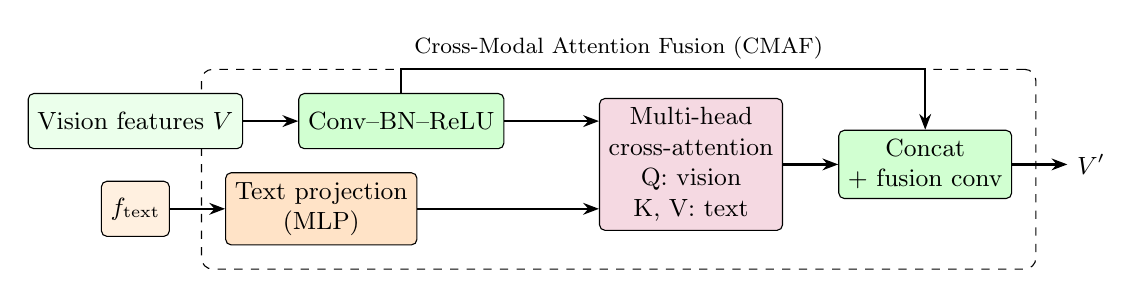
\begin{tikzpicture}[
  font=\small,
  box/.style={draw, rounded corners=2pt, align=center, minimum height=7mm, fill=#1},
  box/.default=white,
  arr/.style={-{Stealth[length=2mm]}, thick},
  node distance=4mm and 7mm]
  \node[box=green!8] (v) {Vision features $V$};
  \node[box=green!18, right=of v] (vc) {Conv--BN--ReLU};
  \node[box=orange!12, below=of v] (t) {$f_{\text{text}}$};
  \node[box=orange!22, right=of t] (tp) {Text projection\\(MLP)};
  \node[box=purple!15, right=12mm of vc, yshift=-5.5mm, minimum height=14mm] (mha)
      {Multi-head\\cross-attention\\Q: vision\\K, V: text};
  \node[box=green!18, right=of mha] (fc) {Concat\\+ fusion conv};
  \node[right=of fc] (o) {$V'$};
  \draw[arr] (v) -- (vc);
  \draw[arr] (t) -- (tp);
  \draw[arr] (vc.east) -- (mha.west |- vc.east);
  \draw[arr] (tp.east) -- (mha.west |- tp.east);
  \draw[arr] (mha) -- (fc);
  \draw[arr] (vc.north) -- ++(0,3mm) -| (fc.north);
  \draw[arr] (fc) -- (o);
  \begin{scope}[on background layer]
    \node[draw, dashed, rounded corners, inner sep=3mm, fit=(vc)(tp)(mha)(fc),
          label={[font=\footnotesize]above:Cross-Modal Attention Fusion (CMAF)}] {};
  \end{scope}
\end{tikzpicture}
\caption{Top: overview of the framework. Visual attention from CLIP is combined with text-derived
features through cross-modal attention to produce a segmentation mask. Bottom: one CMAF block.}
\label{fig:architecture}
\end{figure}

\subsection{Backbone design}
CLIP consists of a vision encoder and a text encoder, which we treat differently.
\begin{itemize}
  \item \textbf{Text encoder (frozen).} The text encoder is kept completely frozen. Pre-trained on
  large-scale image--text data, it already captures rich semantic relationships between language and
  visual concepts (e.g.\ ``glasses'', ``face mask''). Fine-tuning it on a small task-specific dataset
  risks catastrophic forgetting; freezing it preserves its ability to generalise across phrasings.
  \item \textbf{Vision encoder (partially fine-tuned).} Only the final transformer blocks of the vision
  encoder are set as trainable. Early layers capture low-level, transferable features such as edges and
  textures, whereas deeper layers encode higher-level semantics better suited to adaptation. This lets
  the model specialise while retaining the robustness of pre-trained features and reducing overfitting
  and compute.
\end{itemize}

\subsection{Role of attention maps}
CLIP embeddings are a global representation of the whole image, well suited to classification but
insufficient for segmentation, which needs spatial localisation. Attention maps preserve spatial
information: the CLS token attends to image patches, and the attention weights indicate the relative
importance of each region. We use these maps as an initial estimate of the occluded region.

\subsection{Visual attention extraction}
We extract attention from the final transformer layer of the visual encoder, focusing on the
interaction between the CLS token and the image patches. This gives a tensor
$a \in \mathbb{R}^{B \times H \times N}$, where $H$ is the number of heads and $N$ the number of
patches. We average over heads, reshape to a spatial grid and upsample to the input resolution:
\begin{equation}
  A_{\text{vis}} = \operatorname{Upsample}\!\left(\frac{1}{H}\sum_{h=1}^{H} a^{(h)}\right).
\end{equation}
The resulting map is a coarse spatial prior over regions of interest.

\subsection{Text feature representation}
From the text encoder we extract a compact vector that summarises attention patterns across tokens.
Instead of using the full embedding, we aggregate CLS-to-token attention from each of the last three
layers into one scalar per layer, giving $f_{\text{text}} \in \mathbb{R}^{3}$. This vector acts as the
semantic signal that guides segmentation.

\subsection{Cross-Modal Attention Fusion}
To combine visual and textual information we use a Cross-Modal Attention Fusion (CMAF) module.
Conceptually, visual features indicate \emph{where} relevant regions are, and text features indicate
\emph{what} the model should focus on. Cross-attention, with spatial vision tokens as queries and the
projected text feature as key and value, lets the model refine visual attention using semantic cues:
\begin{equation}
  V' = \operatorname{Fusion}\big(V,\ \operatorname{CrossAttention}(V, f_{\text{text}})\big).
\end{equation}

\subsection{Segmentation head}
The head refines the visual attention map through three convolutional stages, each followed by a CMAF
block (channel flow $1 \to 128 \to 64 \to 128 \to 64 \to 64 \to 64 \to 1$). Spatial resolution is kept
fixed while the features are progressively refined. A final $1\times1$ convolution and sigmoid output a
single-channel mask in $[0,1]$.

\subsection{Dice loss}
In occlusion segmentation the foreground is typically much smaller than the background, and losses
such as binary cross-entropy that weigh every pixel equally can perform poorly under this imbalance.
Dice loss measures overlap directly:
\begin{equation}
  \mathcal{L}_{\text{Dice}} = 1 - \frac{2\,TP + \epsilon}{2\,TP + FP + FN + \epsilon}.
\end{equation}
It decreases as overlap increases, penalises both false positives and false negatives, focuses on
region-level rather than per-pixel agreement, and handles class imbalance naturally.

% ---------------------------------------------------------------------------
\section{Experiments}

\subsection{Implementation details}
All experiments use CLIP ViT-B/32 from OpenAI's \texttt{clip} library. Images are pre-processed with
CLIP's default pipeline (resize to $224\times224$, normalise); masks are resized to $224\times224$ and
binarised at 0.5. Training runs on a single NVIDIA GPU, with checkpoints saved every two epochs.
Table~\ref{tab:hparams} lists the hyperparameters.

\begin{table}[h]
  \centering
  \caption{Training hyperparameters.}
  \label{tab:hparams}
  \begin{tabular}{ll}
    \toprule
    Hyperparameter & Value \\
    \midrule
    CLIP backbone & ViT-B/32 \\
    Image size & $224\times224$ \\
    Batch size & 24 \\
    Optimiser & AdamW \\
    Learning rate & $1\times10^{-4}$ \\
    Weight decay & 0.01 \\
    Epochs & 50 \\
    Train / val split & 80\% / 20\% \\
    Dice loss smoothing $\epsilon$ & 1.0 \\
    Text layers used & 3 \\
    CMAF hidden dim & 64 \\
    Segmentation head hidden channels & 128 \\
    \bottomrule
  \end{tabular}
\end{table}

\subsection{Training curves}
Figure~\ref{fig:dice} shows the Dice loss of saved checkpoints across training, and
Table~\ref{tab:dice} reports it at selected epochs.

\begin{figure}[h]
  \centering
  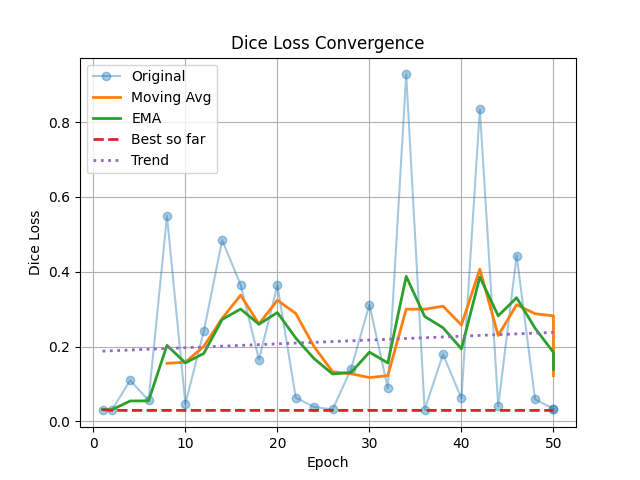
\includegraphics[width=0.7\linewidth]{dice_loss_convergence.png}
  \caption{Dice loss across the 50 training epochs, with moving average, exponential moving average,
  best-so-far and linear trend.}
  \label{fig:dice}
\end{figure}

\begin{table}[h]
  \centering
  \caption{Dice loss ($\downarrow$) at selected training epochs.}
  \label{tab:dice}
  \begin{tabular}{cc}
    \toprule
    Epoch & Dice loss \\
    \midrule
    6 & 0.0559 \\
    10 & 0.0468 \\
    18 & 0.1650 \\
    22 & 0.0633 \\
    24 & 0.0383 \\
    50 & 0.0336 \\
    \bottomrule
  \end{tabular}
\end{table}

\subsection{Segmentation results: CelebA and LFW}
We evaluate on a held-out subset of CelebA and on LFW~\cite{huang2008lfw} to assess generalisation to
an unseen distribution, using mean Intersection over Union:
\begin{equation}
  \text{mIoU} = \frac{1}{N}\sum_{i=1}^{N} \frac{|P_i \cap G_i|}{|P_i \cup G_i|},
\end{equation}
where $P_i$ and $G_i$ are the predicted and ground-truth binary masks for sample $i$. Ground-truth masks
for evaluation are generated with MediaPipe facial landmarks. Table~\ref{tab:miou} reports the scores.

\begin{table}[h]
  \centering
  \caption{mIoU on held-out test sets.}
  \label{tab:miou}
  \begin{tabular}{lcl}
    \toprule
    Dataset & mIoU & Notes \\
    \midrule
    CelebA (held-out) & 0.9441 & In-distribution \\
    LFW & 0.9405 & Out-of-distribution \\
    \bottomrule
  \end{tabular}
\end{table}

The model achieves an mIoU of 0.9441 on held-out CelebA and 0.9405 on LFW. The small gap between
in-distribution and out-of-distribution performance suggests good generalisation, which we attribute
to the frozen CLIP text encoder's semantic representations and the prompt augmentation used during
training.

\subsection{Qualitative analysis}
Figure~\ref{fig:qualitative} shows example LFW inputs with the CLS-token attention map, the predicted
mask and the ground truth. The raw CLIP attention is spatially diffuse and centred broadly on prominent
facial features; the segmentation head reshapes it towards the occluded region named in the prompt.

\begin{figure}[h]
  \centering
  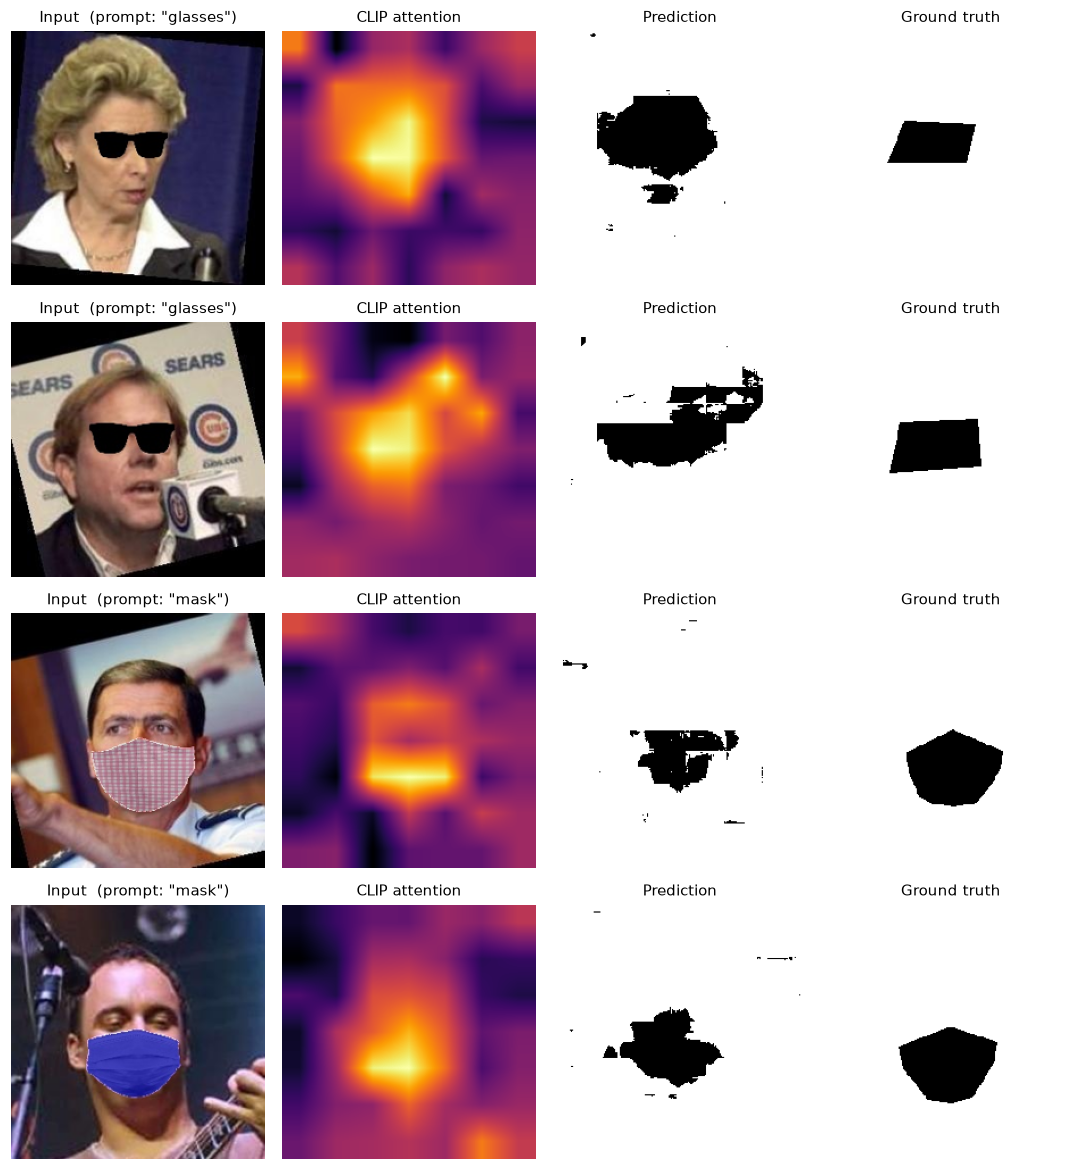
\includegraphics[width=0.85\linewidth]{qualitative.png}
  \caption{Qualitative results on LFW. Columns: input image with prompt, CLS-token attention map,
  predicted mask, ground truth (occluded region shown in black).}
  \label{fig:qualitative}
\end{figure}

% ---------------------------------------------------------------------------
\section{Discussion}

\paragraph{Freezing strategy.}
Keeping the text encoder frozen is important: it has already learned precise semantic representations
of occlusion categories, and fine-tuning it on a small task-specific dataset risks degrading them.

\paragraph{Compact text representation.}
The text feature $f_{\text{text}} \in \mathbb{R}^{3}$ is deliberately minimal: it encodes only per-layer
CLS attention statistics rather than the full 512-dimensional CLIP text embedding. This was motivated by
parameter efficiency, but it is a potential bottleneck; richer text representations may improve
performance.

\paragraph{Dice loss for class imbalance.}
Glasses and face masks typically cover a small fraction of the face image. Binary cross-entropy can be
dominated by the majority class in this setting, whereas Dice loss directly optimises overlap between
prediction and ground truth.

% ---------------------------------------------------------------------------
\section{Conclusion}

We presented a lightweight, language-guided face occlusion segmentation framework that repurposes the
internal attention of a pre-trained CLIP model. By combining CLS-token visual attention maps with
compact multi-layer text attention statistics through learned cross-modal fusion modules, the system
segments glasses and face-mask occlusions without a heavy decoder or full backbone fine-tuning, and
reaches an mIoU of 0.9441 on CelebA and 0.9405 on LFW.

\paragraph{Limitations and future work.}
The text representation is very compact ($\mathbb{R}^3$); richer encodings such as the full
512-dimensional CLIP text embedding may improve segmentation quality. The approach uses prompt
augmentation at training time but does not explore zero-shot generalisation to unseen occlusion
categories. Data augmentation (random crops, photometric jitter) and more principled prompt engineering
could improve generalisation, and extending the framework to multi-class occlusion segmentation and
evaluating on benchmarks such as the AR face database would provide broader validation.

\paragraph{Acknowledgments.}
We acknowledge the CelebA and LFW datasets, OpenAI's CLIP library, MaskTheFace and MediaPipe.

% ---------------------------------------------------------------------------
\begin{thebibliography}{99}\small
\bibitem{radford2021clip} A.~Radford, J.~W. Kim, C.~Hallacy, et al. Learning transferable visual models from natural language supervision. \emph{ICML}, 2021.
\bibitem{dosovitskiy2021vit} A.~Dosovitskiy, L.~Beyer, A.~Kolesnikov, et al. An image is worth 16x16 words: Transformers for image recognition at scale. \emph{ICLR}, 2021.
\bibitem{caron2021dino} M.~Caron, H.~Touvron, I.~Misra, et al. Emerging properties in self-supervised vision transformers. \emph{ICCV}, 2021.
\bibitem{luddecke2022clipseg} T.~L\"uddecke and A.~Ecker. Image segmentation using text and image prompts. \emph{CVPR}, 2022.
\bibitem{ronneberger2015unet} O.~Ronneberger, P.~Fischer, and T.~Brox. U-Net: Convolutional networks for biomedical image segmentation. \emph{MICCAI}, 2015.
\bibitem{long2015fcn} J.~Long, E.~Shelhamer, and T.~Darrell. Fully convolutional networks for semantic segmentation. \emph{CVPR}, 2015.
\bibitem{zheng2021setr} S.~Zheng, J.~Lu, H.~Zhao, et al. Rethinking semantic segmentation from a sequence-to-sequence perspective with transformers. \emph{CVPR}, 2021.
\bibitem{chefer2021interpretability} H.~Chefer, S.~Gur, and L.~Wolf. Transformer interpretability beyond attention visualization. \emph{CVPR}, 2021.
\bibitem{selvaraju2017gradcam} R.~R. Selvaraju, M.~Cogswell, A.~Das, et al. Grad-CAM: Visual explanations from deep networks via gradient-based localization. \emph{ICCV}, 2017.
\bibitem{wang2020masked} Z.~Wang, Z.~Huang, and S.~Gong. Masked face recognition dataset and application. arXiv:2003.09093, 2020.
\bibitem{song2019occlusion} L.~Song, D.~Gong, Z.~Li, et al. Occlusion robust face recognition based on mask learning with pairwise differential siamese network. \emph{ICCV}, 2019.
\bibitem{strudel2021segmenter} R.~Strudel, R.~Garcia, I.~Laptev, and C.~Schmid. Segmenter: Transformer for semantic segmentation. \emph{ICCV}, 2021.
\bibitem{xu2022groupvit} J.~Xu, S.~De Mello, S.~Liu, et al. GroupViT: Semantic segmentation emerges from text supervision. \emph{CVPR}, 2022.
\bibitem{ren2024groundedsam} T.~Ren, S.~Liu, A.~Zeng, et al. Grounded SAM: Assembling open-world models for diverse visual tasks. arXiv:2401.14159, 2024.
\bibitem{huang2008lfw} G.~B. Huang, M.~Ramesh, T.~Berg, and E.~Learned-Miller. Labeled Faces in the Wild: A database for studying face recognition in unconstrained environments. UMass Amherst Technical Report 07-49, 2007.
\bibitem{liu2015celeba} Z.~Liu, P.~Luo, X.~Wang, and X.~Tang. Deep learning face attributes in the wild. \emph{ICCV}, 2015.
\bibitem{anwar2020maskedface} A.~Anwar and A.~Raychowdhury. Masked face recognition for secure authentication. arXiv:2008.11104, 2020.
\bibitem{lugaresi2019mediapipe} C.~Lugaresi, J.~Tang, H.~Nash, et al. MediaPipe: A framework for building perception pipelines. arXiv:1906.08172, 2019.
\bibitem{liang2023ovseg} F.~Liang, B.~Wu, X.~Dai, et al. Open-vocabulary semantic segmentation with mask-adapted CLIP. \emph{CVPR}, 2023.
\end{thebibliography}

\end{document}
